\begin{figure}[htbp]
\section*{ HMGCS2}
\centering
\begin{subfigure}[b]{0.95\textwidth}
\centering
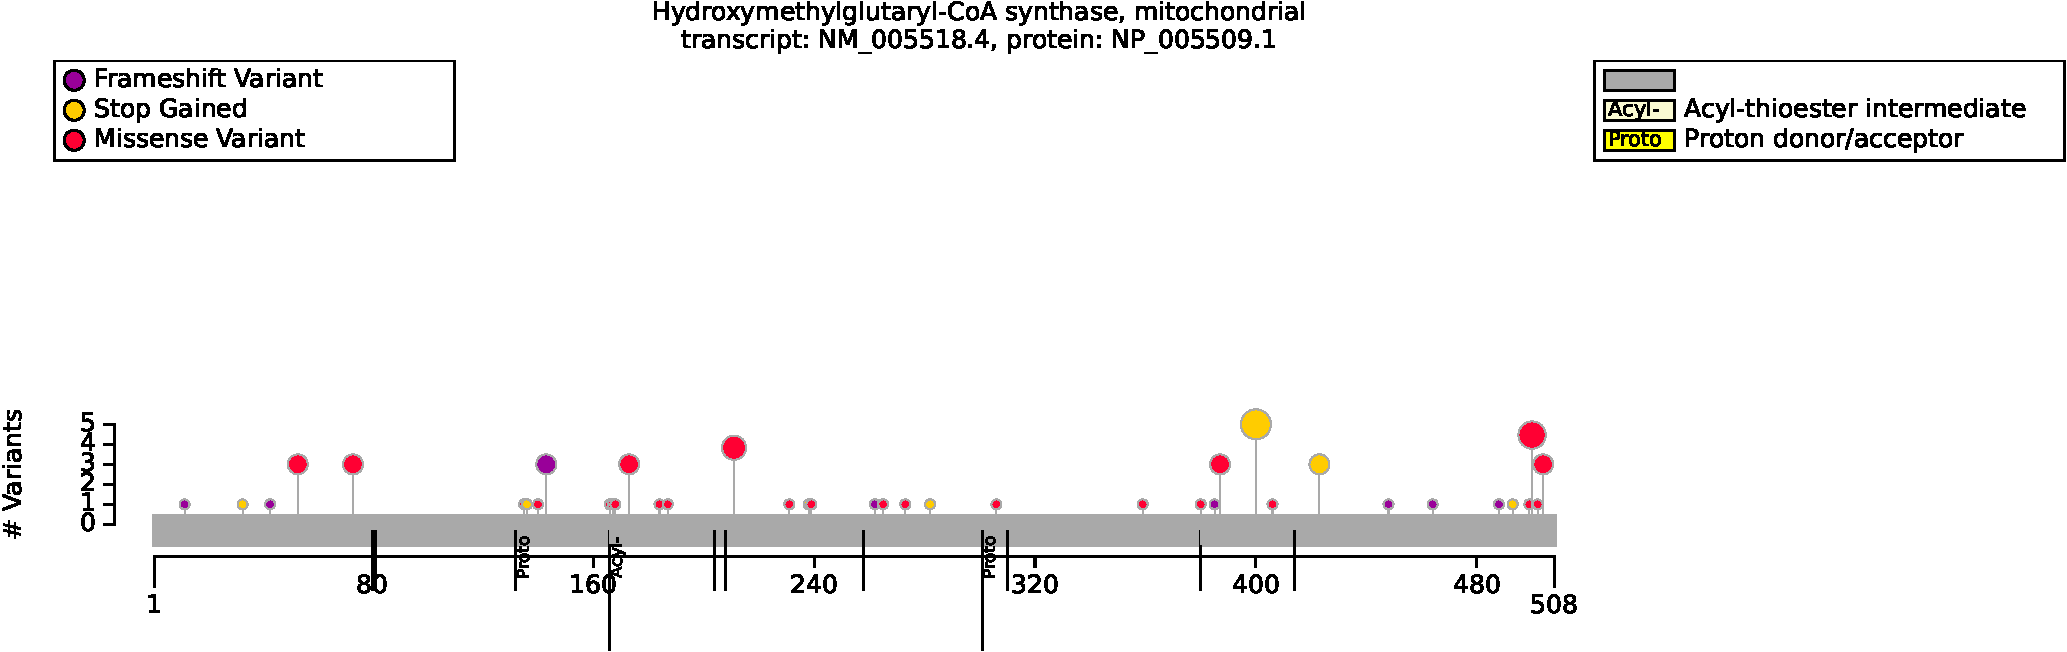
\includegraphics[width=\textwidth]{ img/HMGCS2_protein_diagram.pdf} 
\captionsetup{justification=raggedright,singlelinecheck=false}
\caption{Distribution of variants in HMGCS2}
\end{subfigure}

\vspace{2em}

\begin{subfigure}[b]{0.35\textwidth}
    \centering
    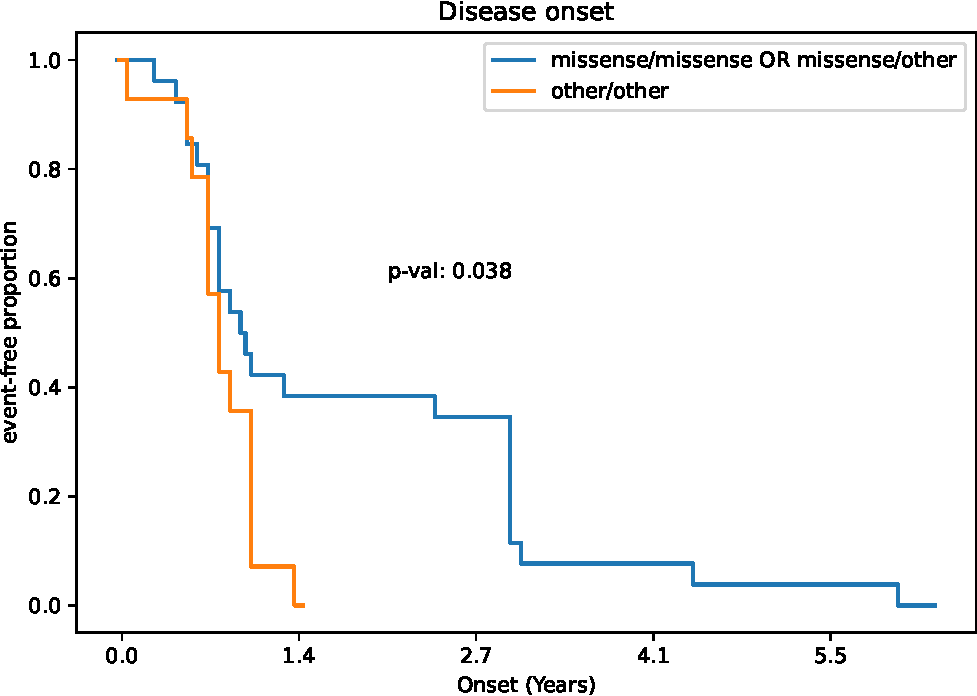
\includegraphics[width=\textwidth]{ img/HMGCS2_stats.pdf} 
    \captionsetup{justification=raggedright,singlelinecheck=false}
    \caption{Onset of HMGCS2 for missense/missense and missense/other vs. other/other variants.}
    \end{subfigure}
    
    \vspace{2em}

\begin{subfigure}[b]{0.95\textwidth}
\centering
\resizebox{\textwidth}{!}{
\begin{tabular}{llllrr}
\toprule
Genotype (A) & Genotype (B) & total tests performed & significant results\\
\midrule
missense/missense OR missense/other & other/other & 19 & 0\\
missense/missense OR missense/other & other/other & 19 & 0\\
FEMALE & MALE & 17 & 0\\
\bottomrule
\end{tabular}
}
\captionsetup{justification=raggedright,singlelinecheck=false}
\caption{Fisher Exact Test performed to compare HPO annotation frequency with respect to genotypes. }
\end{subfigure}

\vspace{2em}

\begin{subfigure}[b]{0.95\textwidth}
\captionsetup{justification=raggedright,singlelinecheck=false}
\resizebox{\textwidth}{!}{
\begin{tabular}{llllrr}
\toprule
Description & Variable & Genotype (A) & Genotype (B) & p-value & xrefs\\
\midrule
HMG-CoA synthase-2 deficiency (OMIM:605911) disease onset & Onset of OMIM:605911 & missense/missense OR missense/other & other/other & 0.038 & -\\
\bottomrule
\end{tabular}
}
\caption{ Onset of OMIM:605911 to compare missense/missense OR missense/other and other/other with respect to Onset of OMIM:605911. }
\end{subfigure}

\vspace{2em}

\caption{The cohort comprised 40 individuals (14 females, 13 males, 13 with unknown sex). 1 of these individuals were reported to be deceased. A total of 44 HPO terms were used to annotate the cohort. Disease diagnosis: HMG-CoA synthase-2 deficiency (OMIM:605911). No previous publications with results on genotype-phenotype correlations in HMGCS2 were identified. A total of 46 unique variant alleles were found in \textit{HMGCS2} (transcript: \texttt{NM\_005518.4}, protein id: \texttt{NP\_005509.1}).}
\end{figure}
